\section{Normalized Cross-Correlation based segmentation}\label{P1}

Template matching, also known as intensity patch matching, is utilized in this section of the assignment in order to identify the black and red cars that are present in a film that has six separate snapshots. It is important to note that the location of the red automobile does not undergo a significant amount of change over the many snapshots of the video. On the other hand, the position and orientation of the black car shifts as it turns left, making its recognition more difficult in comparison to the detection of the red car. One of the approaches that is utilized in order to accomplish this objective (template matching) is known as "Normalized Cross-Correlation," which is a method that is more reliable in comparison to the methodology of raw cross correlation. The degree of resemblance between two signals or images that are located at separate places can be determined through the use of cross-correlation. We calculate a similarity score at each place by sliding the template or patch over the larger image and then calculating the score. When there are differences in intensity, contrast, and lighting between the template and the region in the bigger image, normalization is utilized to ensure that these differences are maintained. Because of this, the approach is more resistant to changes in both the illumination and the contrast. It is expected that a perfect match will be located someplace in the picture with the highest score, which is the spot in the score map that is the brightest (value equal to 1).


\[
\hat{f} = \frac{f - \bar{f}}{\sqrt{\sum (f - \bar{f})^2}}, \quad
\hat{g} = \frac{g - \bar{g}}{\sqrt{\sum (g - \bar{g})^2}}
\]

\[
NCC(f, g) = C_{fg}(\hat{f}, \hat{g}) = \sum_{[i,j] \in R} \hat{f}(i, j)\hat{g}(i, j)
\]

Regarding the initial section, the patch is chosen in such a manner that it encompasses the entirety of the automobile. The procedure is carried out once more for both the red and the black of the cars. If one were to possess the size of the patch and be aware of the location of the highest score, which is represented by a red dot, it would be feasible to identify the automobile in the photo, which is represented by a rectangle surrounding the automobile. The patches for the red and black automobiles are depicted in Figures 1 and 3, respectively, and the red and black cars that were found in the six photographs are depicted in Figures 2 and 4.


\begin{figure} [ht]
    \centering
    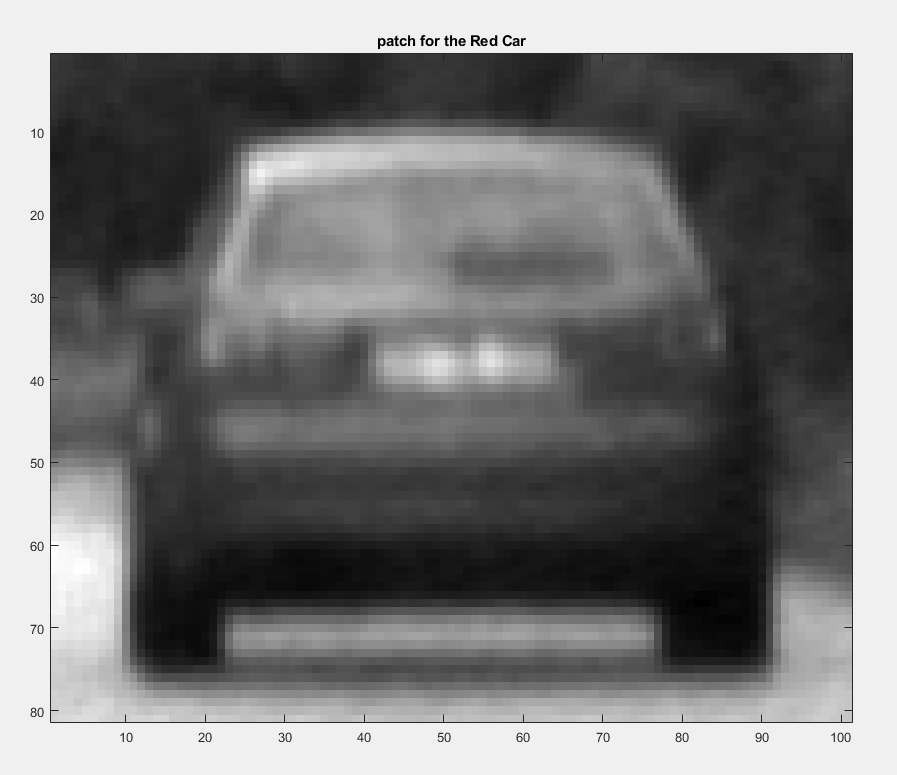
\includegraphics[width = 0.5\textwidth]{Resources/F1.png}
    \caption{The patch to detect the Red car}
    \label{fig:The patch to detect the Red car}
\end{figure}

\begin{figure} [ht]
    \centering
    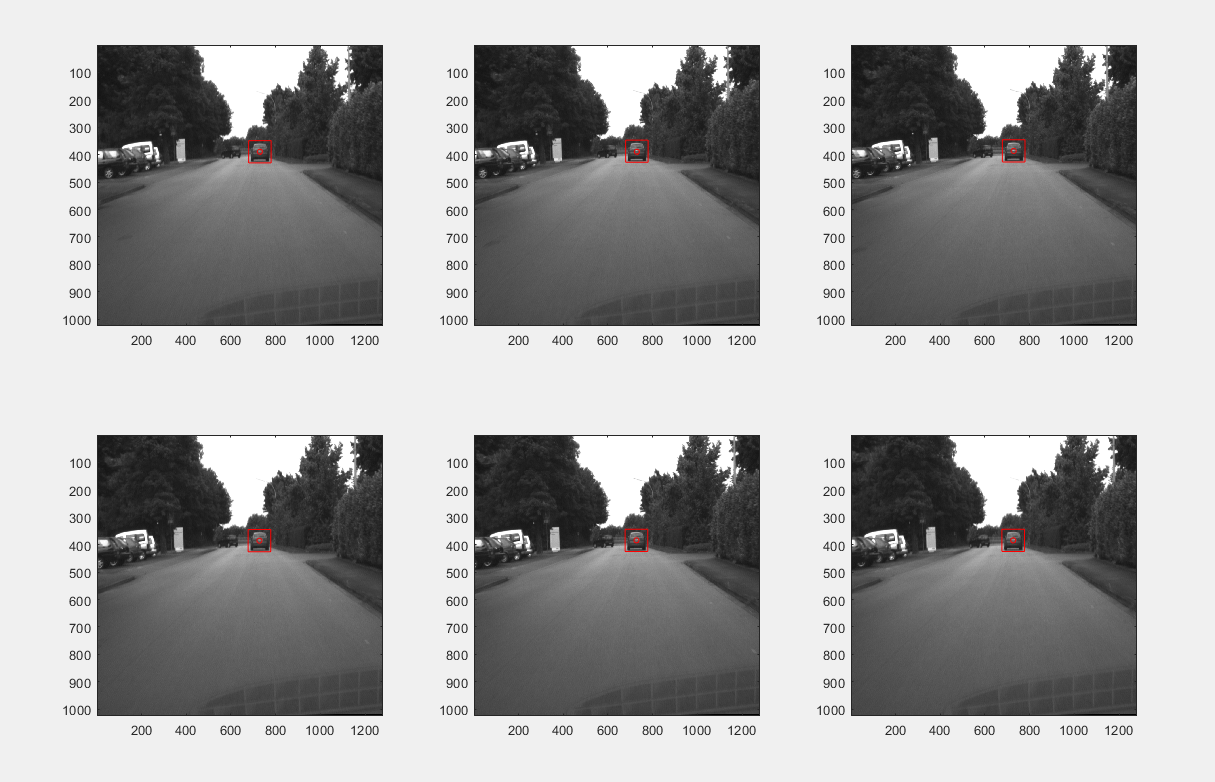
\includegraphics[width = 0.9\textwidth]{Resources/F2.png}
    \caption{6 pictures in which the Red car has been detected}
    \label{fig:6 pictures in which the Red car has been detected}
\end{figure}

\begin{figure} [!]
    \centering
    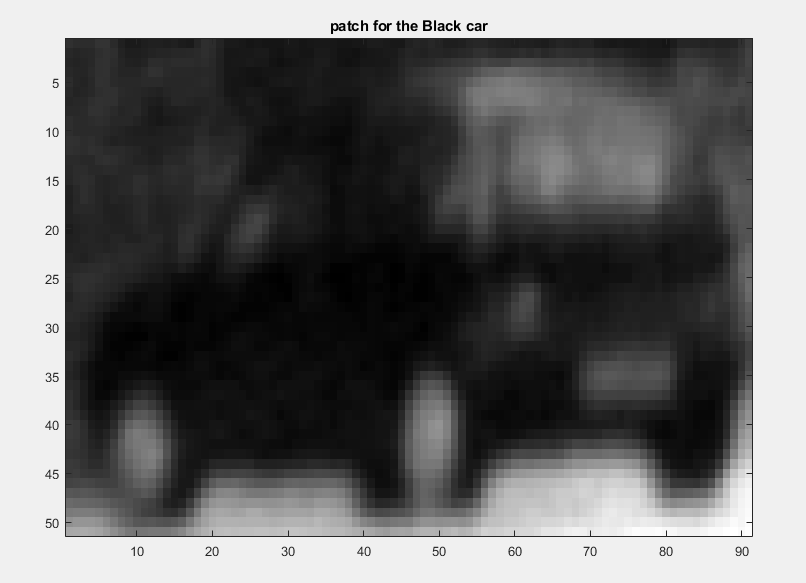
\includegraphics[width = 0.5\textwidth]{Resources/F3.png}
    \caption{The patch to detect the Black car}
    \label{fig:The patch to detect the Black car}
\end{figure}

\begin{figure} [h]
    \centering
    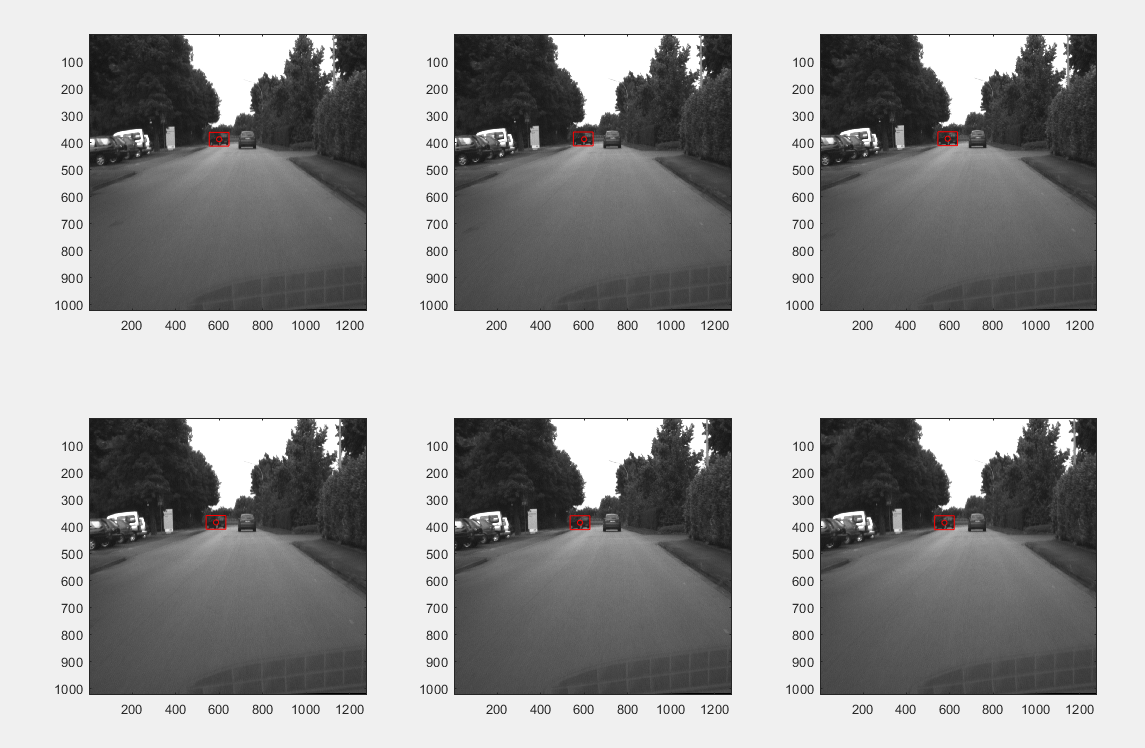
\includegraphics[width = 0.9\textwidth]{Resources/F4.png}
    \caption{6 pictures in which the Black car has been detected in each.}
    \label{fig:6 pictures in which the Black car has been detected in each.}
\end{figure}

When utilizing this strategy, it is evident that both red and black automobiles are identified with a high degree of precision being achieved. As a result of a small portion of the automobile's front not being positioned within the rectangle, there is only a slight imperfection in the detection of the black car in the most recent snapshot of the image.
"Color based segmentation" is an additional technique that can be utilized to identify an object in a photograph. This technique is based on the colors of the object being analysed. First, it is required to select the region that encompasses the color spectrum of the object that is to be detected. This is the technique that requires you to follow. The "Hue" values from the HSV color space representation, along with the calculation of the mean and the standard deviation of the "H" parameter, make it feasible to have a mask that defines a range in order to literally compare the colors and identify the objects when they are present. Both the red and black autos will require the same procedure to be repeated. Both in terms of computing efficiency and ease of implementation, the color-based segmentation method is a good choice. This can be helpful in situations where the items of interest have colors that are both distinct and consistent. The fact that this approach is mostly reliant on the color of objects, however, means that it may be sensitive to changes in lighting conditions, shadows, and differences in the look of items. It is also possible that it will struggle when the background and the objects in the scene have similar colors. The objects that were identified using this method are depicted in Figures 5 and 4, respectively. The template-based strategy is clearly superior to the color-based method in terms of accuracy for this application. This is a fact that cannot be denied. Because the color of the red car is distinct in comparison to the surrounding environment, color-based segmentation has been successful in identifying the vehicle with the required level of precision. It is only able to detect the red portion of the car, and it is unable to detect the entire area surrounding the vehicle, including the tires and the mirrors. The tires and other components of the vehicle have color space properties that are distinct from those of the body of the vehicle, which is the reason given for this phenomenon.

\begin{figure} [ht]
    \centering
    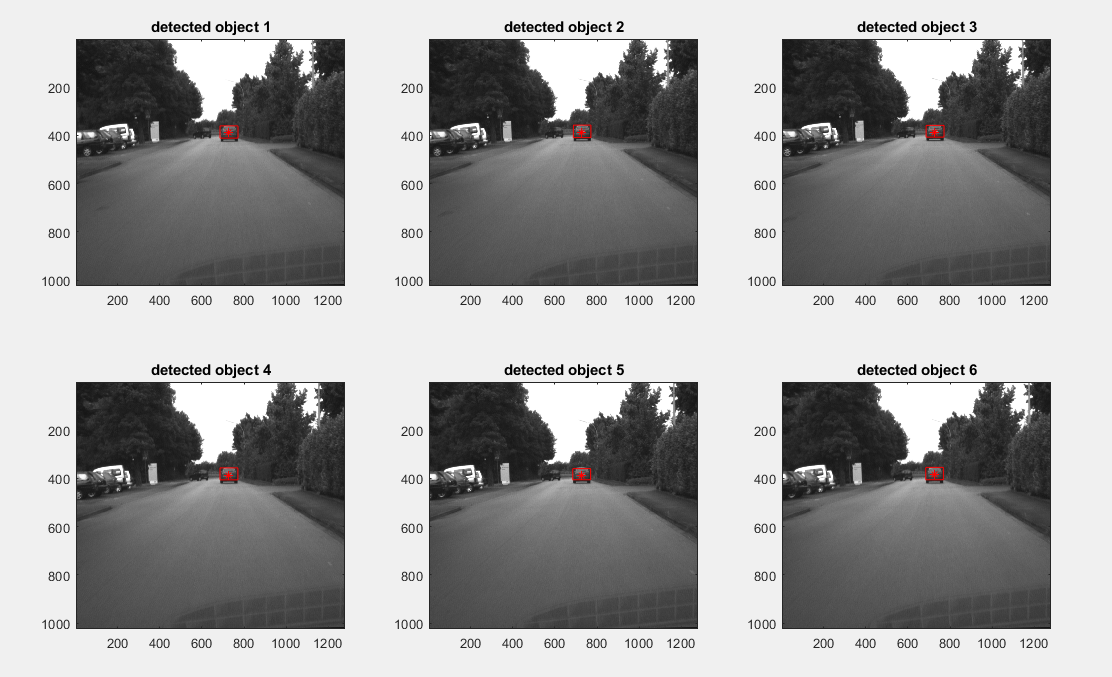
\includegraphics[width = 0.9\textwidth]{Resources/F5.png}
    \caption{6 pictures in which the Red car has been detected in each with color-based detection.}
    \label{fig:6 pictures in which the Red car has been detected in each with color-based detection.}
\end{figure}

When the color-based segmentation and template matching methods are used to the black automobile, it is clear that the color-based segmentation method has not been able to accurately detect the entire contour of the car's body. One of the primary reasons for this is because the color spectrum of the car is very close to the background and area in which it is located. The alteration in the position and appearance of the car is still another basis for the shift. When it comes to this particular application, template matching might be recommended as the strategy that yields the most accurate results.


\begin{figure} [ht]
    \centering
    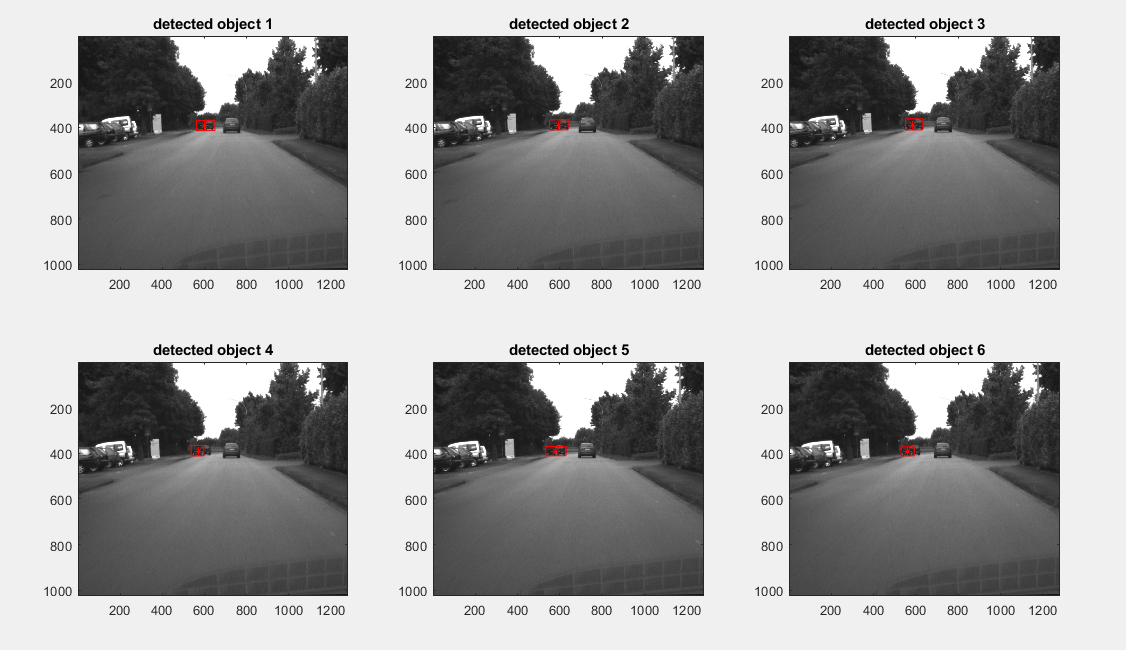
\includegraphics[width = 0.9\textwidth]{Resources/F6.png}
    \caption{6 pictures in which the Black car has been detected in each with color-based detection.}
    \label{fig:6 pictures in which the Black car has been detected in each with color-based detection.}
\end{figure}

\par
When it comes to comparison, there are a number of different characteristics that may be taken into consideration during the process. A total of three windows are defined in such a way that the smallest one is a perfect fit for the automobile, the next one is somewhat larger, and the final one contains a significantly larger number of pixels that encompass both the automobile and the neighborhood that surrounds it. The findings indicate that the process will become more time-consuming as the frame of the patch continues to grow in size; however, the accuracy will be relatively enhanced as a result of this time investment. This may be owing to the fact that larger patches contain a greater number of pixels, and matching larger patches requires comparing a greater number of pixels, which results in an increase in the amount of time required for computing. It is also possible that they will demand additional memory for processing and storage. By increasing the size of the window, the estimation becomes more accurate and resilient to changes in the rotation and lighting of the object. This is because the window gives more information. However, it may reveal certain data that are not necessary and may display some sections of the image that are not necessary as the item that has been spotted. As a result, it can appear to be more advantageous to use the highest score point as a criterion for comparing accuracy. As a consequence of this, it is possible to comprehend that the greatest score point will be more accurate when the frame is a perfect fit for the object, in contrast to when larger frames are utilized; nonetheless, as the position of the car shifts, certain components of the automobile are not positioned within the detected region. To get a successful match, it is essential to strike a balance between the size of the patch and the qualities of the objects or features that we are attempting to replicate. Because of this, we will be able to arrive at a more accurate figure within the allotted amount of time. The following images provide an accurate illustration of the effect that increasing the patch size has (Figure 4 depicts the frame that is a perfect match for the automobile).

\begin{figure} [ht]
    \centering
    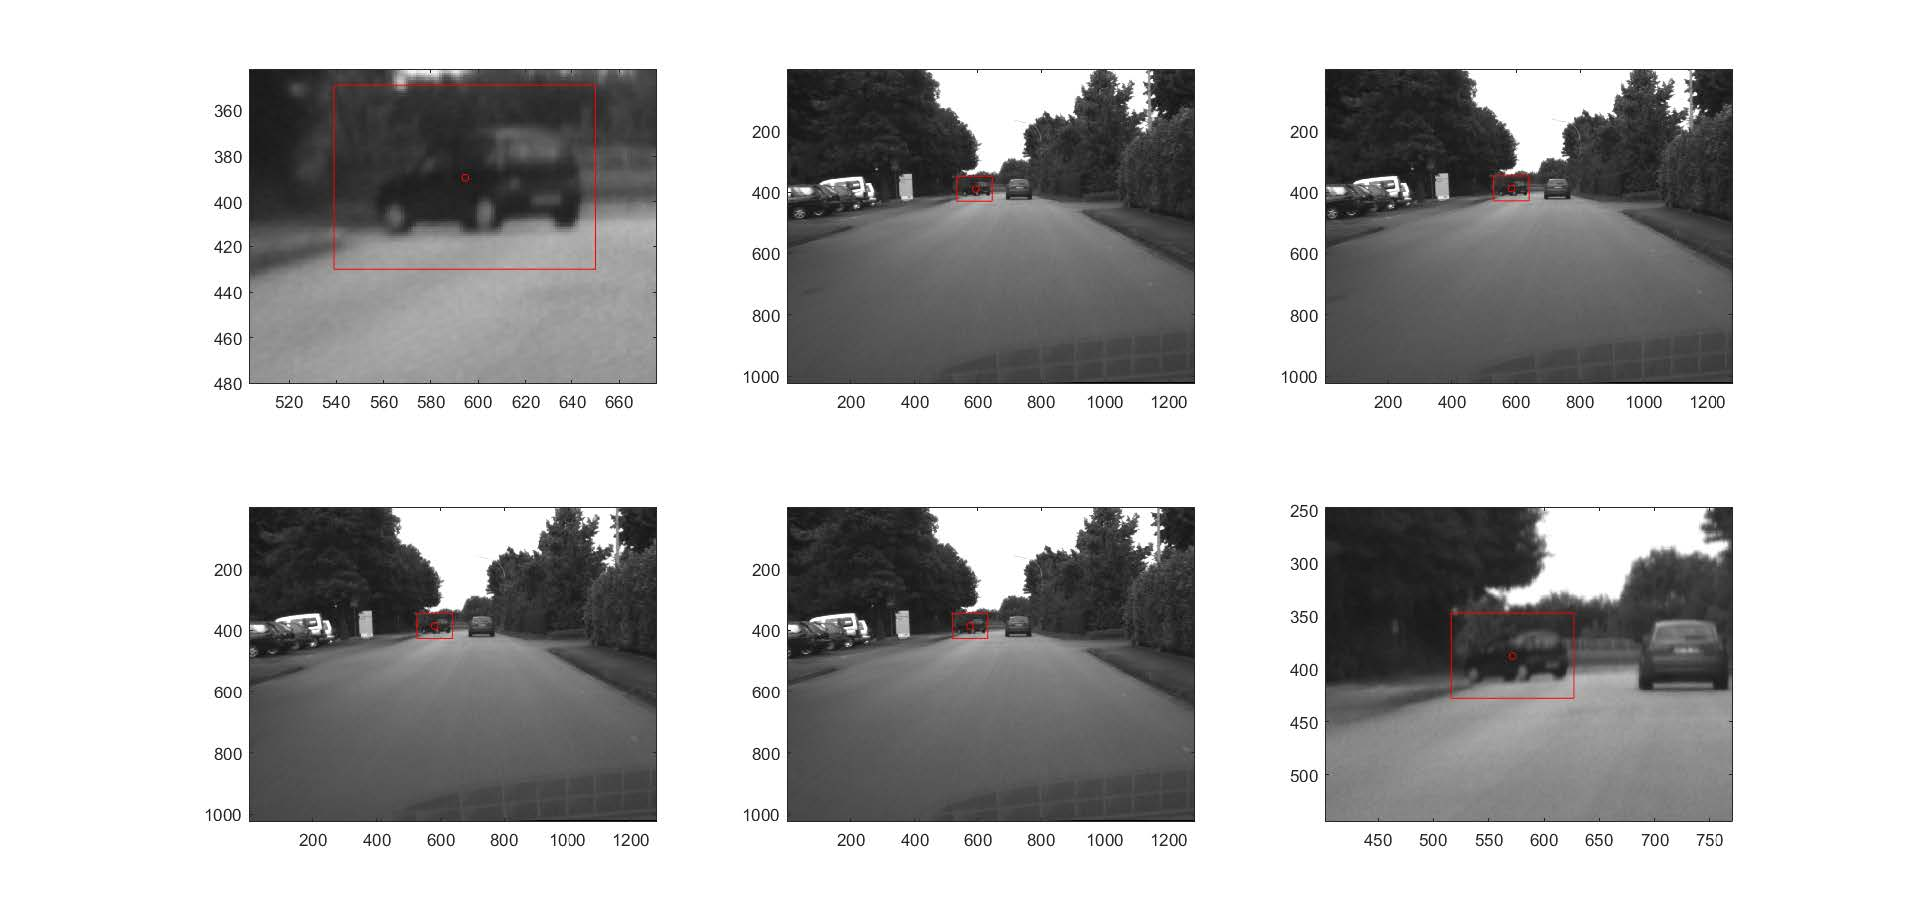
\includegraphics[width = 0.9\textwidth]{Resources/F7-1.jpg}
    \caption{The first results of detecting objects with larger frames}
    \label{fig:The first results of detecting objects with larger frames}
\end{figure}

\begin{figure} [ht]
    \centering
    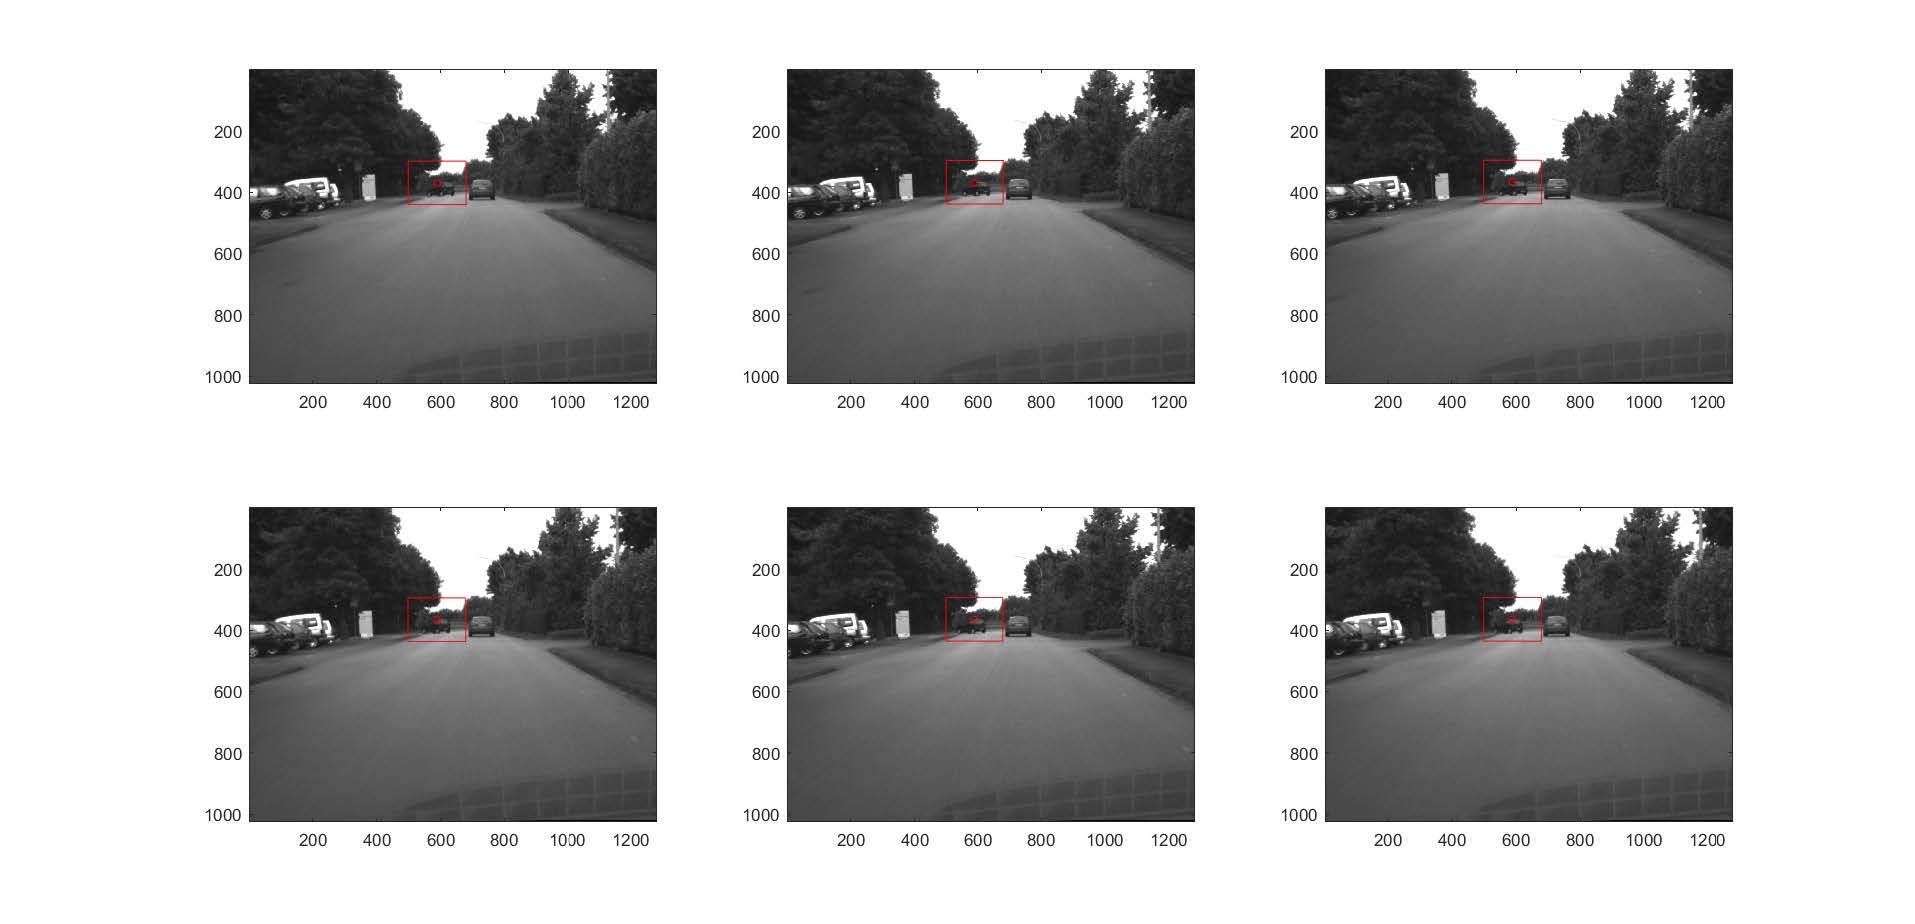
\includegraphics[width = 0.9\textwidth]{Resources/F8-1.jpg}
    \caption{The Second results of detecting objects with larger frames}
    \label{fig:The Second results of detecting objects with larger frames}
\end{figure}